\section{RVV}\label{chap:bg:sec:rvv}
% RISC-V has extensions
RISC-V is an open family of ISAs which defines ``base integer ISAs'' (e.g. all 64-bit RISC-V cores implement the RV64I Base Integer Instruction Set) and extensions (e.g. the ``M'' extension for integer multiplication).
A base instruction set combined with a set of extensions is known as a RISC-V ISA.
Because RISC-V is open, anyone can design, manufacture, and sell chips implementing any RISC-V ISA.
% RVV is the vector one
RVV is the officially ratified vector extension for RISC-V, and going forward all RISC-V chips with vector processing capabilities should implement it instead of designing their own custom vector extensions.
This section is based on the RVV Specification v1.0\todocite{RVV spec 1.0}.

\subsection{Vector model}
RVV defines thirty-two vector registers, each of an implementation-defined width VLEN.
These registers can be interpreted as vectors of varying element sizes, and the largest possible element size is ELEN.
RVV also adds some state that defines how the vector registers are used (see \cref{fig:RVV_added_state}).
% \begin{figure}
%     \centering
%     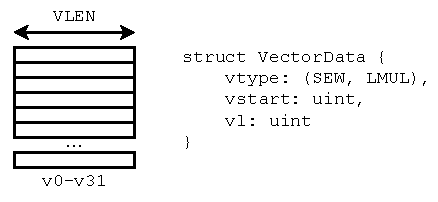
\includegraphics[width=0.7\textwidth]{Figures/RVV_Additions.pdf}
%     \caption{Summary of additional state used by RVV}
%     \label{fig:RVV_added_state}
% \end{figure}
\begin{basicfig}{Figures/RVV_Additions.pdf}
    \caption{Summary of additional state used by RVV}
    \label{fig:RVV_added_state}
\end{basicfig}

\subsubsection{\code{vl} and \code{vstart}}
The first piece of state is the Vector Length \code{vl}, which holds the number of elements that could be updated from a vector instruction.
The program updates this value through fault-only-first loads (\todoref{fof load}) and more commonly the \code{vsetvl} instruction family (\todoref{vsetvl}).

In the simple case, \code{vl} is equal to the total available elements (see \cref{fig:RVV_vl_full}).
It can also be fewer (see \cref{fig:RVV_vl_short}), in which case vector instructions will not write to elements in the \enquote{tail} (i.e. elements past \code{vl}).
This eliminates the need for a `cleanup loop' common in fixed-length vector programs.

\figcheckinputs{}
\expanded{\noexpand\begin{figure}[\figinputPos]}
    \centering
    \begin{subfigure}[b]{\figinputWidth}
        \centering
        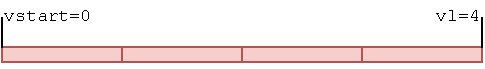
\includegraphics[width=\textwidth]{Figures/RVV_VL_full.pdf}
        \caption{Fully utilized vector}
        \label{fig:RVV_vl_full}
    \end{subfigure}
    \hfill
    \begin{subfigure}[b]{\figinputWidth}
        \centering
        
\includegraphics[width=\textwidth]{Figures/RVV_VL_short.pdf}
        \caption{Partially utilized vector}
        \label{fig:RVV_vl_short}
    \end{subfigure}
    \caption{Examples of vector utilization with \code{vl} and \code{vstart}}
    \label{fig:RVV_vl}
\end{figure}

In a similar vein, \code{vstart} specifies \enquote{the index of the first element to be executed by a vector instruction}.
This is usually only set by the hardware whenever it is interrupted mid-instruction (see \cref{fig:RVV_vstart_trap}) so that the instruction can be re-executed later without corrupting completed values.
The program \emph{can} set this value manually, but it may not always work.
If an implementation couldn't arrive at the value itself, then it is allowed to reject it.
The specification gives an example where a vector implementation never takes interrupts during an arithmetic instruction, so it would never set \code{vstart} during an arithmetic instruction, so it could raise an exception if \code{vstart} was nonzero for an arithmetic instruction.

\begin{figure}
    \centering
    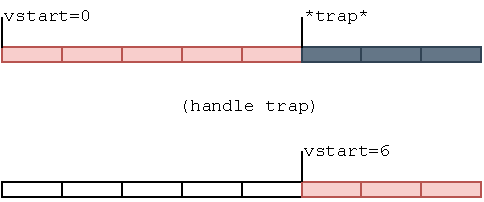
\includegraphics[width=0.7\textwidth]{Figures/RVV_vstart_trap.pdf}
    \caption{Example of the hardware setting \code{vstart} after a trap}
    \label{fig:RVV_vstart_trap}
\end{figure}

\subsubsection{\code{vtype}}
\code{vtype} contains two key fields.
The first is the Selected Element Width (\code{SEW}), which is self-explanatory.
It can be 8, 16, 32, or 64.
Most instructions\footnote{Except where the width is encoded in the instruction, like bytemask loads.} will split vector registers into elements of this width.

The second field is the Vector Register Group Multiplier (\code{LMUL}).
Vector instructions do not necessarily operate over a single register, but over a register \emph{group} as defined by this field.
For example, if \code{LMUL=8} then each instruction would operate over 8 register's worth of elements.
In some implementations this may increase throughput, which by itself is beneficial for applications.

\begin{figure}
    \centering
    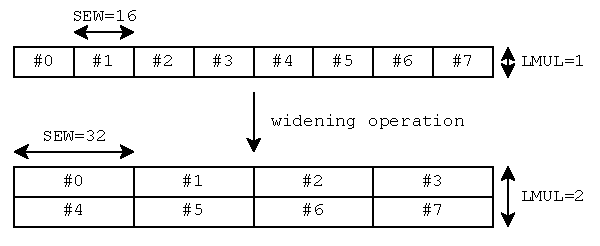
\includegraphics[width=0.7\textwidth]{Figures/RVV_LMUL_Widening.pdf}
    \caption{Example of using LMUL to access results of widening operations}
    \label{fig:RVV_LMUL_widening}
\end{figure}

However, the true utility of \code{LMUL} lies in widening/narrowing operations (see \cref{fig:RVV_LMUL_widening}).
For example, an 8-by-8-bit multiplication can produce 16-bit results.
Because the element size doubles, the number of vector registers required to hold the same number of elements also doubles.
Doubling \code{LMUL} after such an operation allows subsequent instructions to handle all the results at once.

\code{vtype} also encodes two flags: mask-agnostic and tail-agnostic.
If these are set, the implementation is \emph{allowed} to overwrite any masked-out or tail elements with all 1s.

\subsubsection{Masking}
Most vector instructions allow for per-element \emph{masking} (see \cref{fig:RVV_mask_example}).
When masking is enabled, register \code{v0} acts as the `mask register', where each bit corresponds to an element in the vector.
If the mask bit is 1, that element will be `masked out' and not written to (or depending on the mask-agnostic setting, overwritten with 1s).

\begin{figure}
    \centering
    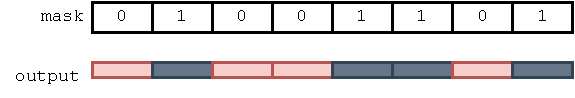
\includegraphics[width=0.8\textwidth]{Figures/RVV_Mask_example.pdf}
    \caption{Example of masking a vector operation}
    \label{fig:RVV_mask_example}
\end{figure}

\subsubsection{Summary}
\begin{basicfig}{Figures/RVV_examples_combined.pdf}
    \caption{Combined examples for RVV vector}
    \label{fig:RVV_examples_combined}
\end{basicfig}
\cref{fig:RVV_examples_combined} shows all of the above features used in a single configuration:
\begin{itemize}
    \item The instruction was previously interrupted and restarted, so \code{vstart=2}
    \item Elements are 16-bit
    \item \code{LMUL=4} to try and increase throughput
    \item Only 29 of the 32 available elements were requested, so \code{vl=29}
    \item Some elements are masked out (in this case seemingly at random)
\end{itemize}

\subsection{Memory accesses}

\subsubsection{Unit + Strided}

\subsubsection{Unit fault-only-first load}
\subsubsection{Unit bytemask load}
\subsubsection{Unit whole-register load}

\subsubsection{Indexed}

\subsection{Interaction with exceptions}

\subsection{Implementations}